\documentclass[../report.tex]{subfiles}
\begin{document}

\graphicspath{{img/}{../img/}}

\subsection{Business Logic Layer Design}

Our design goals for the Business Logic Layer was to make it:
\begin{enumerate}
\item Transparent
\item Supportable
\item Reliable
\item Testable
\end{enumerate}

In order to gain transparency in our Business Logic Layer we decided to use an Abstract Factory pattern with a regular Factory pattern on top to make it possible to gain access to the concrete implementations of the Abstract Factory from outside the Business Logic Layer.

\begin{landscape}

\newgeometry{left=1cm,right=-3cm}

\subsection{Class Diagram}

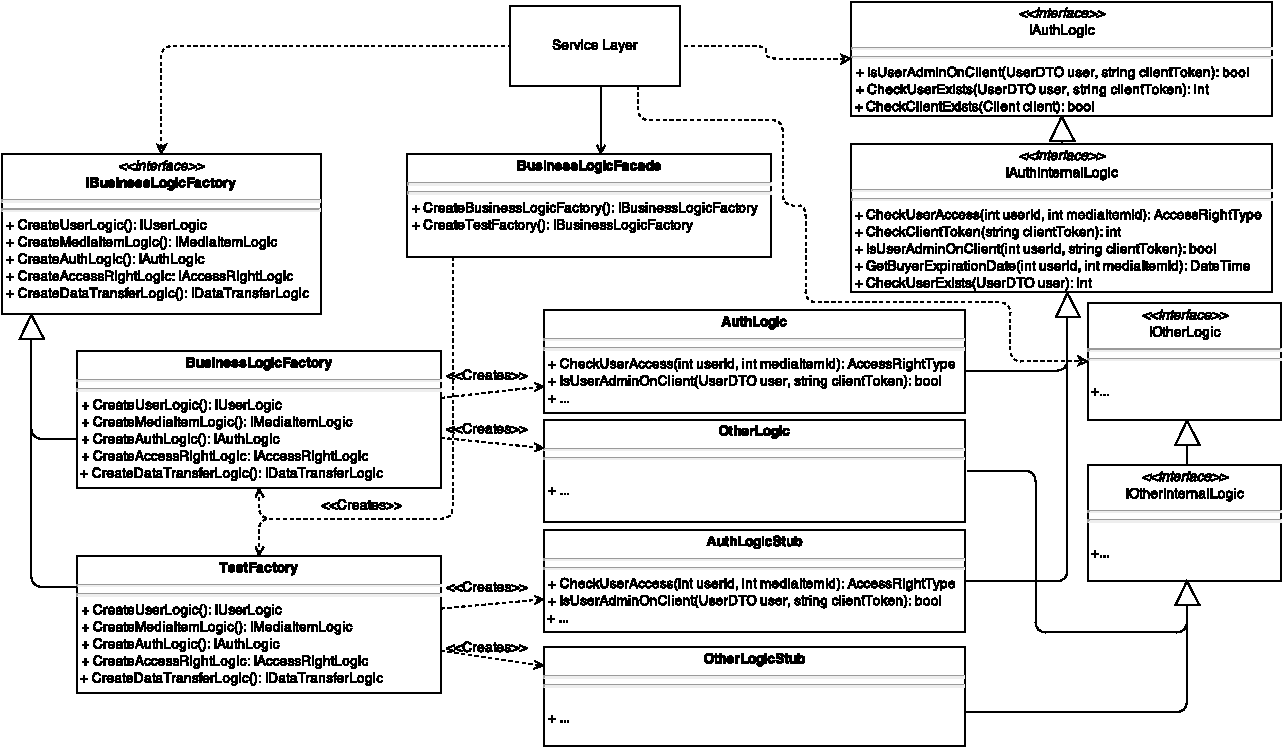
\includegraphics[ scale=1.2]{BusinessLogicLayerDiagram.pdf}

\end{landscape}

The diagram above shows the class structure in the Business Logic Layer. The Entry Factory consists of a single concrete class which in our case is the BusinessLogicEntryFactory class. The BusinessLogicEntryFactory class makes it possible to get hold of the concrete factories without exposing the factories to the Service Layer.

Underneath the Entry Factory lies the Abstract Factory pattern which starts with the Abstract Factory interface which in our case is the IBusinessLogicFactory. This interface specifies a method for creating each of the Abstract Products in this Abstract Factory. The Abstract Products are IAuthLogic, IUserLogic, IMediaItemLogic, IAccessRightLogic and IDataTransferLogic. We then have two concrete implementations of this interface and those are the BusinessLogicFactory and the TestFactory classes. Each of the concrete factories can then produce an instance of a concrete implementation of each Abstract Product. These concrete implementations must implement the Abstract Product interface which contains the methods that are exposed to the Service Layer. But they must also implement an internal interface (ie. IAuthInternalLogic) which specifies methods that are used internally in the Business Logic Layer. These internal interfaces make it possible for the different concrete logic classes to expose methods to one another but not to the Service Layer.

\end{document}